\documentclass[aspectratio=169,usenames,dvipsnames]{beamer}
\beamertemplatenavigationsymbolsempty
% \documentclass{beamer}

% UNCOMMENT FOR HANDOUTS
% \usepackage{pgfpages}
% \pgfpagesuselayout{2 on 1}[landscape,letterpaper,border shrink=5mm]
% \setbeameroption{show notes}

\mode<presentation>
\usetheme{Boadilla}
\usecolortheme{spruce}
\usepackage{../../LizStyle,ulem}
\usepackage{color}
\usepackage[color,matrix,arrow]{xy}
% \input xy
% \xyoption{all}
\usepackage{tikz}
\usepackage{tikz-cd}
\tikzset{commutative diagrams/diagrams={ampersand replacement=\&}}

\AtBeginSection{\frame{\sectionpage}}


% ==========Command for putting comments and removing them=======
% Visible:
\newcommand{\InstructorNotes}[1]{\textit{\color{orange}#1}}
\newcommand{\InstructorList}[1]{
\begin{itemize}
	\color{orange}
	#1
\end{itemize}
}
% Removed:
% \renewcommand{\InstructorNotes}[1]{}
%\renewcommand{\InstructorList}[1]{}


\newcommand{\bvfill}{\vskip0pt plus 1filll}

\usepackage{multimedia}
\usepackage{graphbox}

% \usepackage{algpseudocode}



\graphicspath{ {Figures/} {../Figures/}{../../Figures/} }



\begin{document}
%\pdfoptionpdfminorversion 5
%\logo{\includegraphics[height=1.5cm]{dukeshield.pdf}}
\title[]{Ch 12.1, 12.4: Unsupervised Learning \& Clustering}
\subtitle{Lecture 32 - CMSE 381}
\date{Mon, Apr 13, 2026}



\institute[MSU-CMSE]{Michigan State University\\
			::\\
          Dept of Computational Mathematics, Science \& Engineering}
%\author[Dr.~Zhang]{Prof.~Mengsen Zhang}

\begin{frame}
 \titlepage


\end{frame}
%--------------------------
\begin{frame}[c]{Announcements }

\begin{columns}
\column{.55\textwidth}
\centering

	\textbf{Last time:}
	\begin{itemize}
	\item Convolutional Neural Nets
	\end{itemize}


	\textbf{This lecture:}
	\begin{itemize}
		\item Clustering (Just hierarchical clustering)
\end{itemize}

\textbf{Announcements:}
	\begin{itemize}
	\item Fri 4/17: Review - submit your questions \href{https://forms.office.com/r/BuaKCT05gG}{here}!
	\item Monday 4/20: Exam 3
	\begin{itemize}
		\item Content since 2nd Exam (Ch 7 and on)
		\item One page (8.5x11) handwritten cheat sheet
		\item no-internet Calculator 
	\end{itemize}

	%\item after: Project office hours, zoom only (link on \href{https://msu-cmse-courses.github.io/CMSE381-S25/Course_Info/Schedule.html\#google-calendar-for-office-hours}{website}).


	\end{itemize}

\column{.35\textwidth}
\centering

	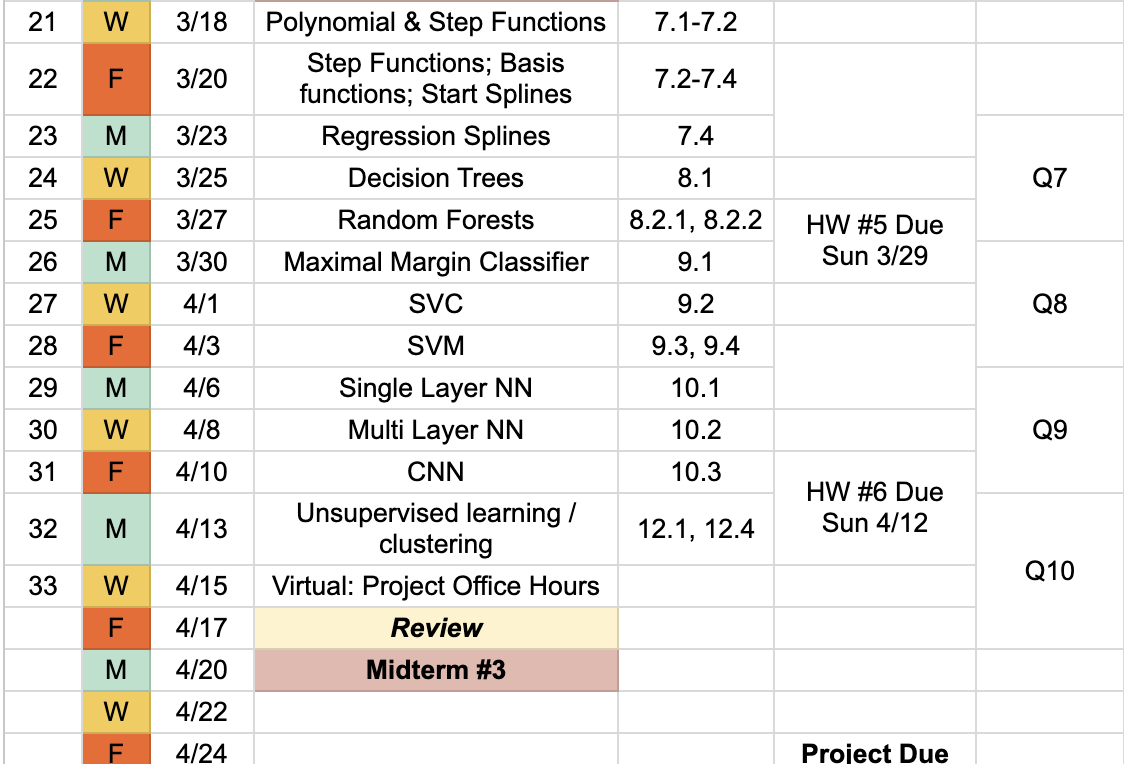
\includegraphics[align = c, width = \textwidth]{Schedule-S26-3.png}

	
\end{columns}

\end{frame}
%--- Next Frame ---%
\begin{frame}[t]{What will you learn today?}

\begin{itemize}
	\item What is the difference between supervised vs unsupervised learning?
	\item What do clustering methods aim to accomplish?
	\item How to interpret a dendrogram of hierarchical clustering? 
	\item How are different linkage methods defined?
	\item How to perform hierarchical clustering in Python? 
\end{itemize}

\end{frame}


%=================
\section{Unsupervised learning}
%=================


\begin{frame}[t]{Supervised vs Unsupervised Learning}

\begin{columns}
\column{.45\textwidth}
\centering
\textbf{Supervised}
\InstructorList{
  \item Have input data
	\item Have output values for the data
	\item Can be regression/classification
	\item Get output values $\hat Y$ and see how close they are to $Y$
}


\column{.45\textwidth}
\centering
\textbf{Unsupervised}

\InstructorList{
  \item no pre-defined output
  \item focus on the relation between predictors or the samples
  \item More subjective
	\item No single/simple goal
	\item Oftenused in \textit{exploratory data analysis}
	\item No universally accepted measure of assessment


}






\end{columns}

\end{frame}
%--- Next Frame ---%


\begin{frame}[t]{Some examples of unsupervised problems}

\begin{columns}
\column{.45\textwidth}
\centering

\begin{itemize}
	\item Assay gene expression levels in 100 patients with breast cancer, looking for subgroups with similar qualities
	\item Online shopping: find groups of shoppers with similar browsing and purchase histories and show relevant related products.
	\item Search engine picking results to show
\end{itemize}


\column{.45\textwidth}
\centering

\end{columns}

\end{frame}
%--- Next Frame ---%
%=================
\section{Clustering}
%=================
\begin{frame}[t]{Big idea}

\begin{columns}
\column{.3\textwidth}
Clustering: relation between samples
\centering
\InstructorList{
  \item Find subgroups or clusters in a data set
  \item Sometimes specify requested number of clusters in advance
	\item Broad class of techniques for this
	\item To do this, need to decide what it means for two data points to be similar or different
}



\column{.65\textwidth}
\centering
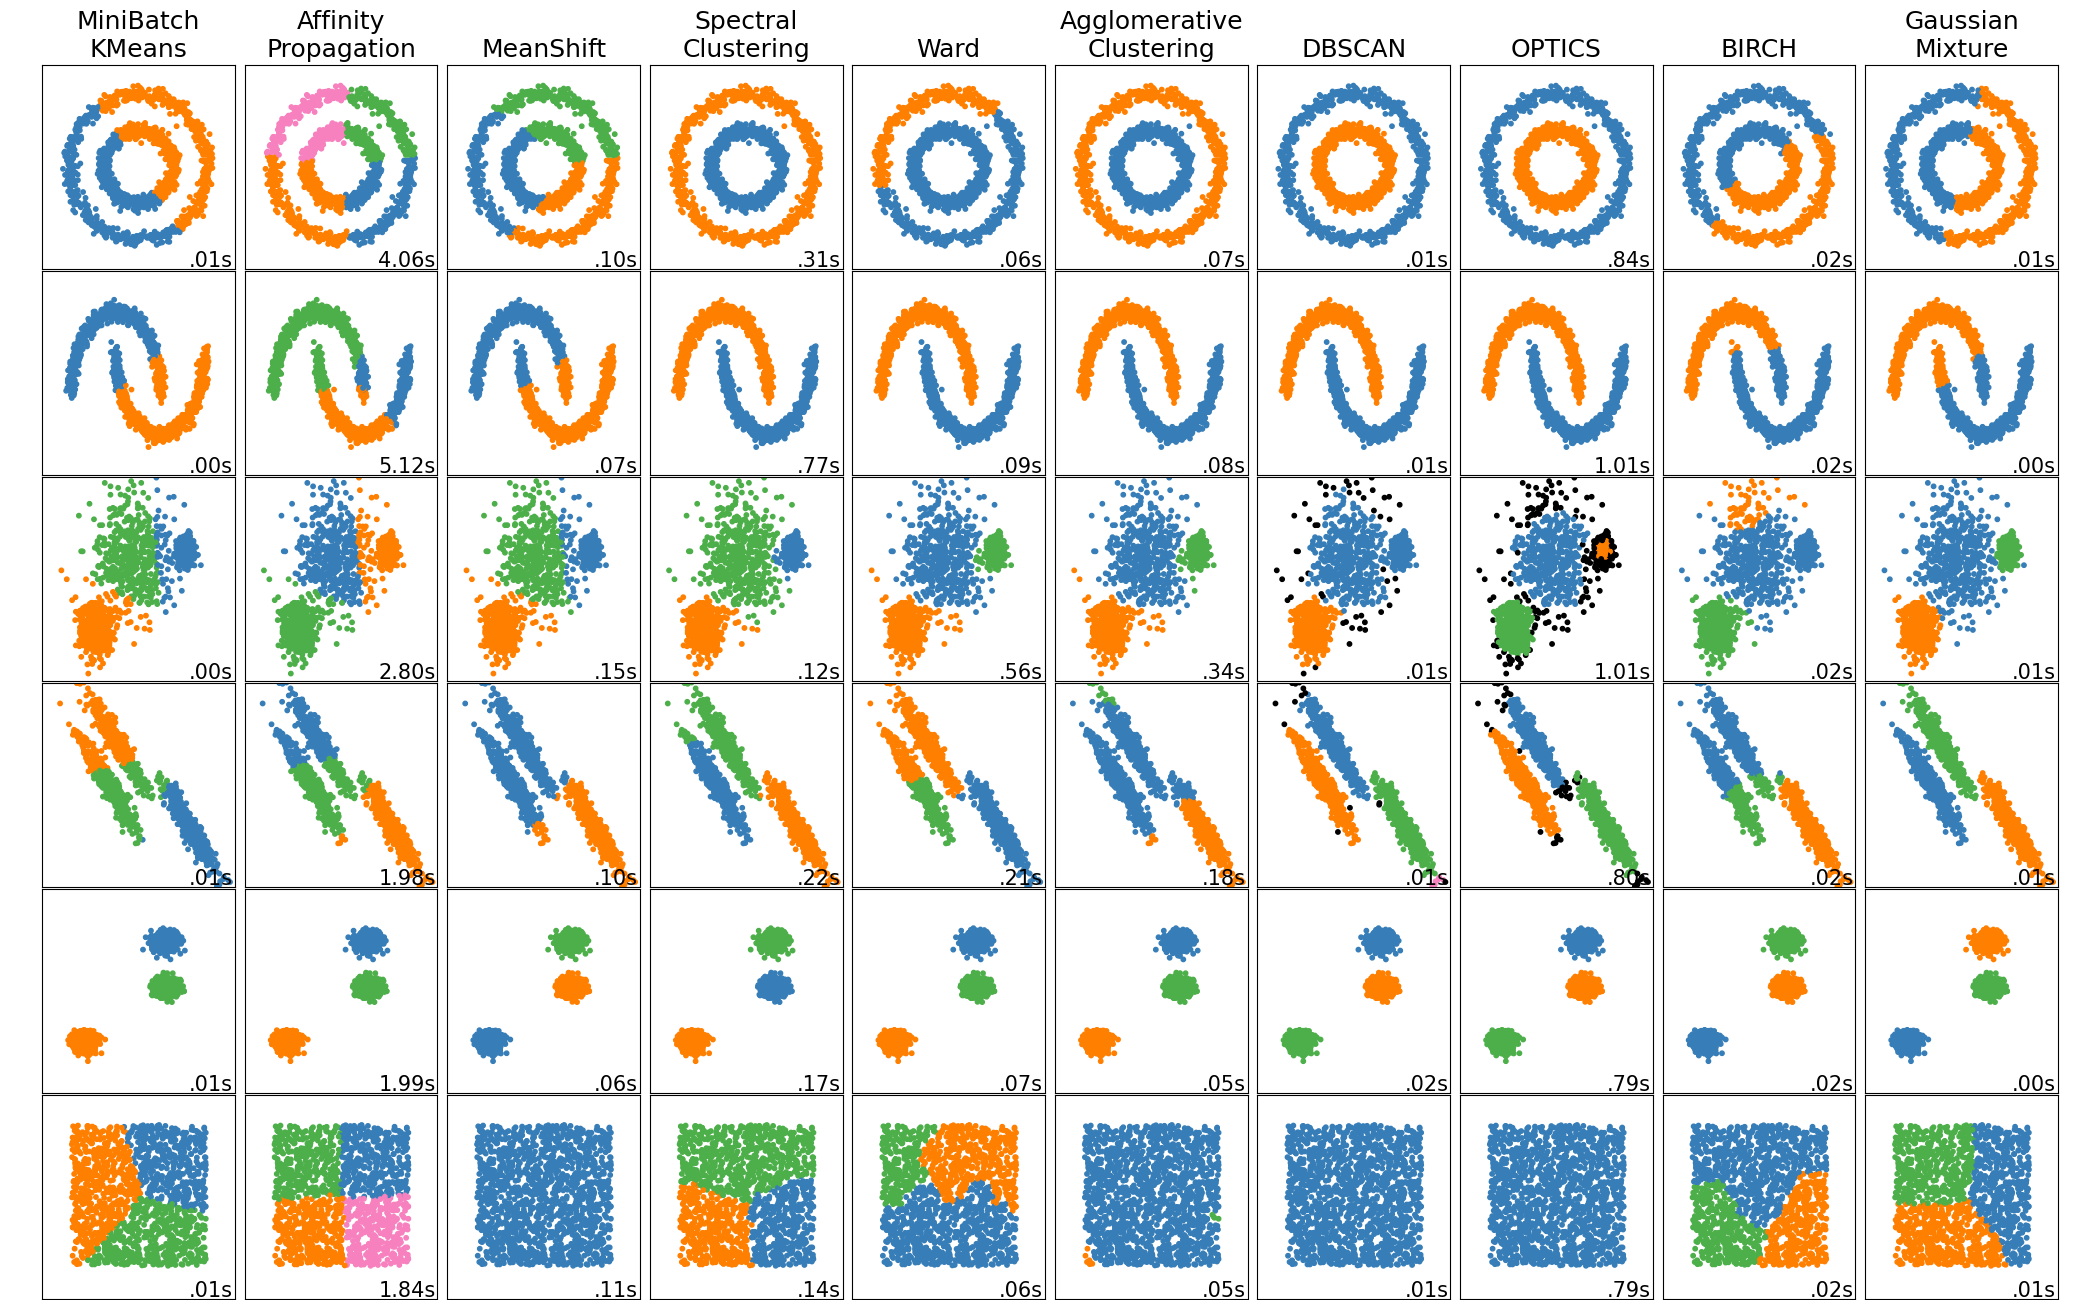
\includegraphics[align = c, width = \textwidth]{sphx_glr_plot_cluster_comparison_001}








\end{columns}

\end{frame}
%--- Next Frame ---%


% %=================
% \section{$K$-Means Clustering}
% %=================





% \begin{frame}[t]{K-Means Clustering}

% \centering
% 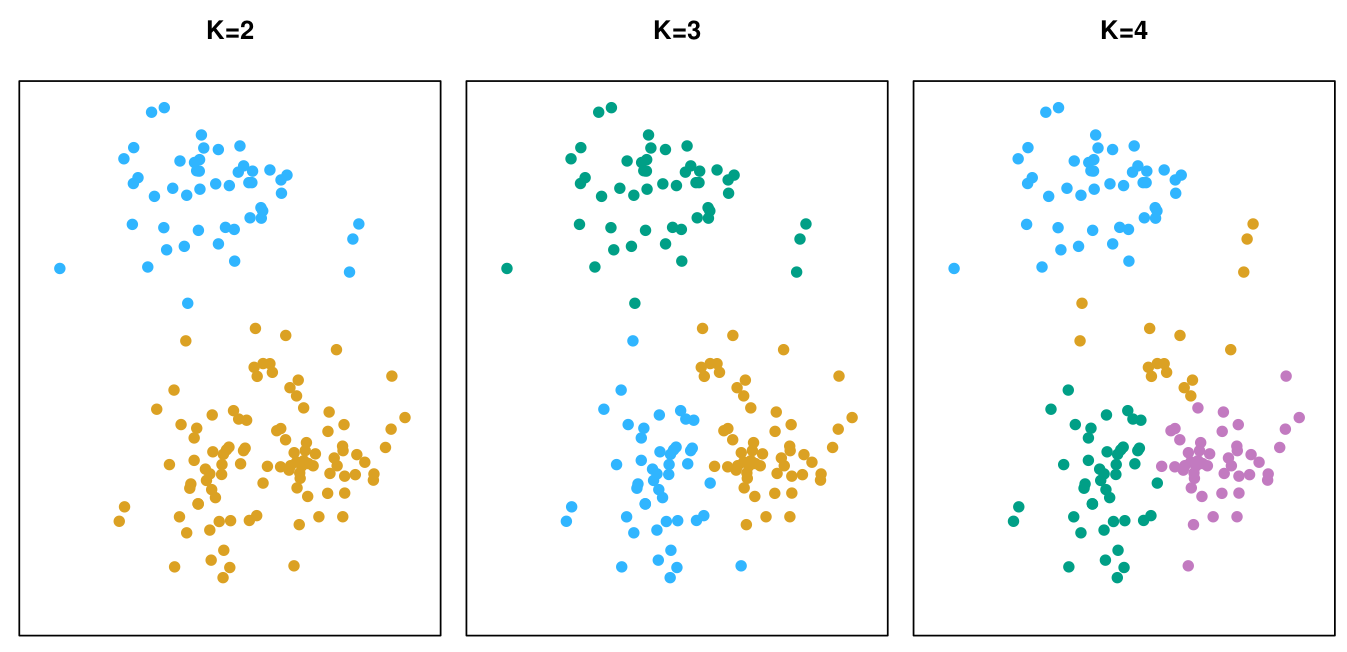
\includegraphics[align = c, width = .65\textwidth]{Fig12-7}
% \InstructorList{
%   \item Partition data into $K$ distinct non-overlapping clusters
% 	\item $K$ needs to be picked in advance
% }
% \begin{columns}
% \column{.25\textwidth}
% \centering



% \column{.65\textwidth}
% \centering





% \end{columns}

% \end{frame}
% %--- Next Frame ---%
% \begin{frame}[t]{Notation}

% \begin{columns}
% \column{.65\textwidth}
% Write sets as $C_1,\cdots,C_K$
% \begin{itemize}
% 	\item $C_1\cup C_2 \cup \cdots C_K = \{1, \cdots,n\}$
% 	\item $C_k \cap C_{k'} = \emptyset$ for all $k \neq k'$
% \end{itemize}
% \column{.25\textwidth}
% \centering
% 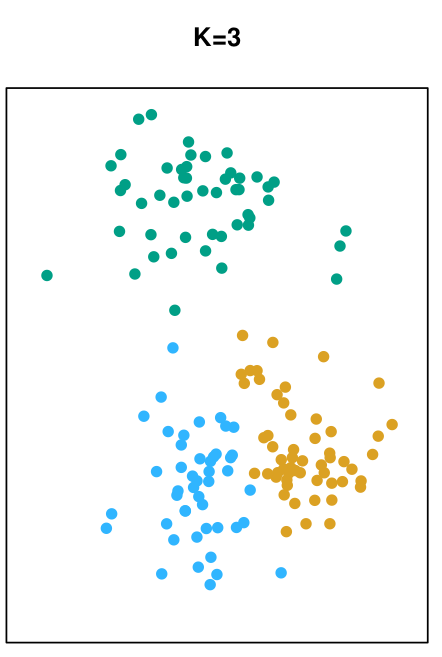
\includegraphics[align = c, width = \textwidth]{Fig12-7b}



% \end{columns}

% \end{frame}
% %--- Next Frame ---%

% \begin{frame}[t]{Good clustering}

% \begin{columns}
% \column{.55\textwidth}
% \centering
% \begin{itemize}
% 	\item
% Goal: within cluster variation is as small as possible\\
% 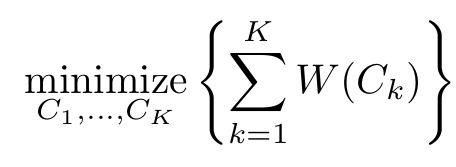
\includegraphics[align = c, width = .5\textwidth]{Eq12-15}

% \item One choice for measuring variation: squared euclidean distance
% 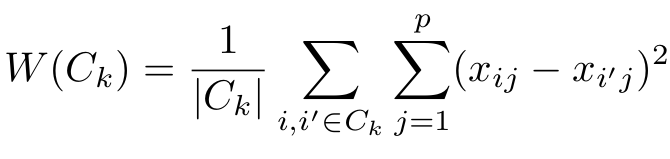
\includegraphics[align = c, width = .8\textwidth]{Eq12-16}


% \end{itemize}








% \column{.25\textwidth}
% \centering

% 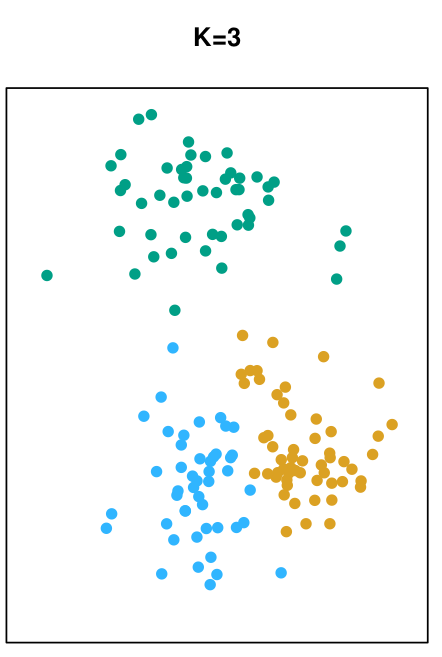
\includegraphics[align = c, width = \textwidth]{Fig12-7b}
% \end{columns}

% \end{frame}
% %--- Next Frame ---%
% \begin{frame}[t]{The problem}

% \begin{columns}
% \column{.45\textwidth}
% \centering
% 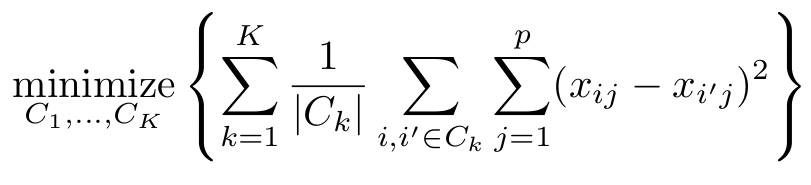
\includegraphics[align = c, width = \textwidth]{Eq12-17}



% \InstructorList{
%   \item Too many partitions to check ($K^n$)
% 	\item Instead, find pretty good (local optimum)
% }



% \column{.45\textwidth}
% \centering
% 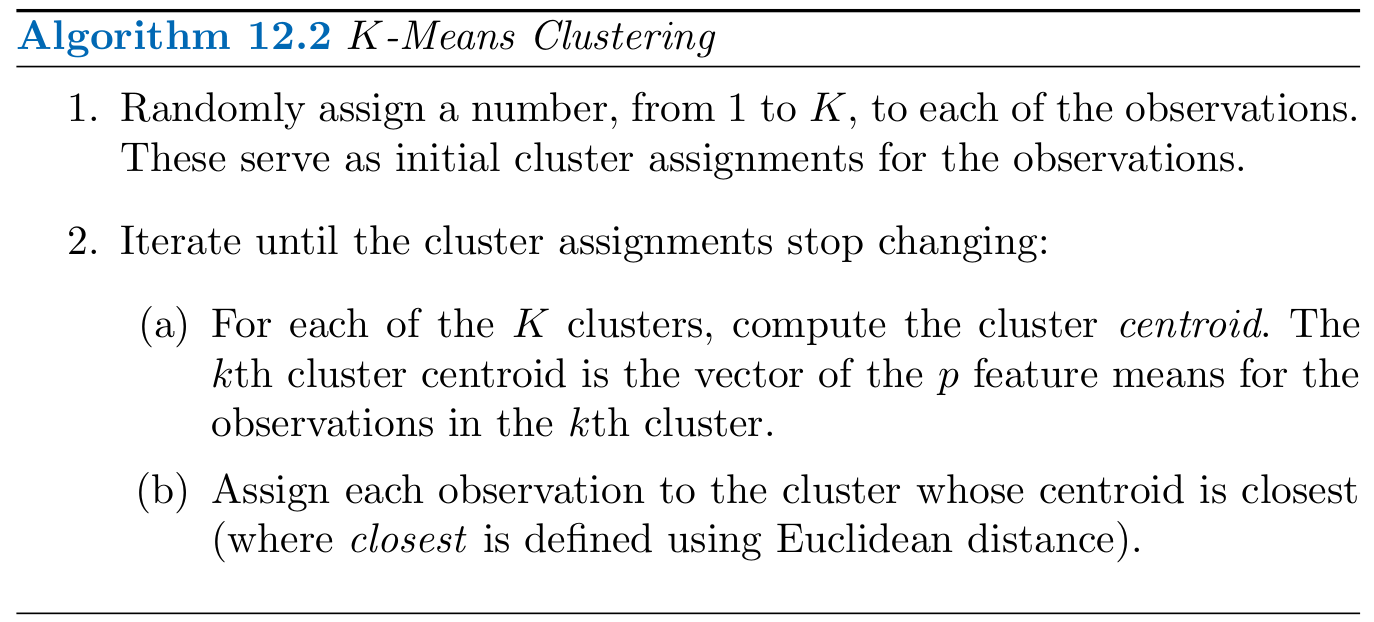
\includegraphics[align = c, width = \textwidth]{Alg12-2}



% \end{columns}


% 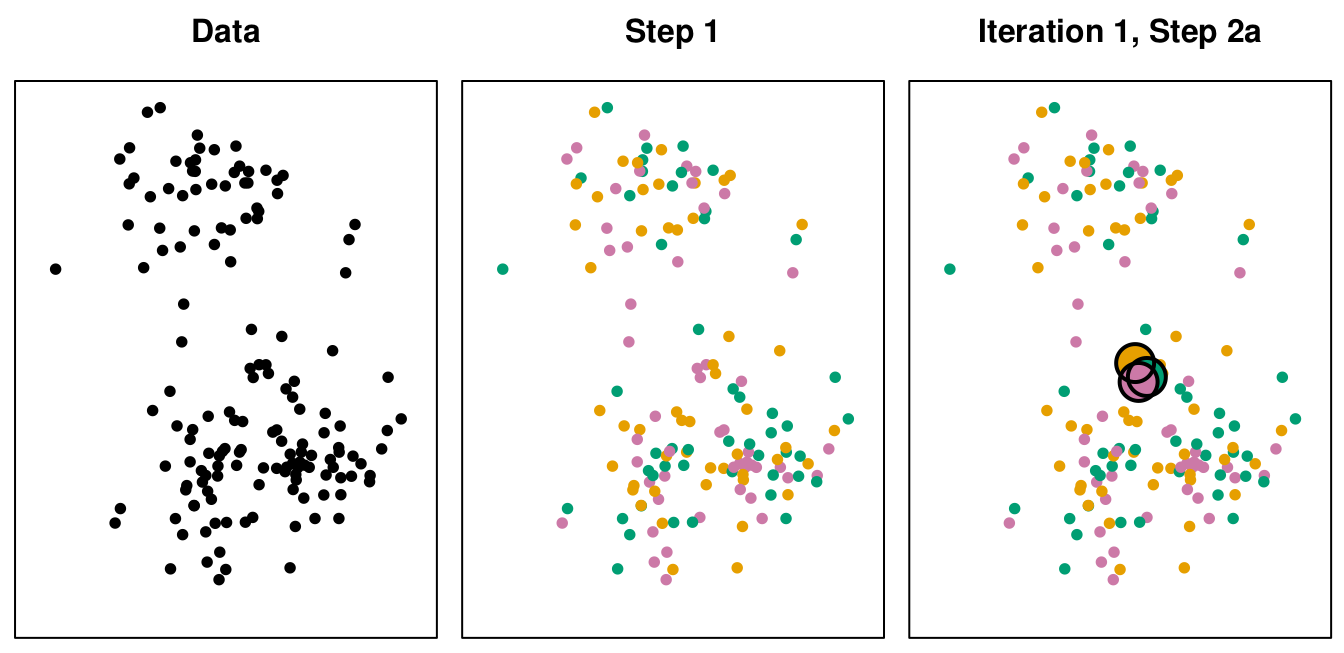
\includegraphics[align = c, width = .45\textwidth]{Fig12-8a}
% 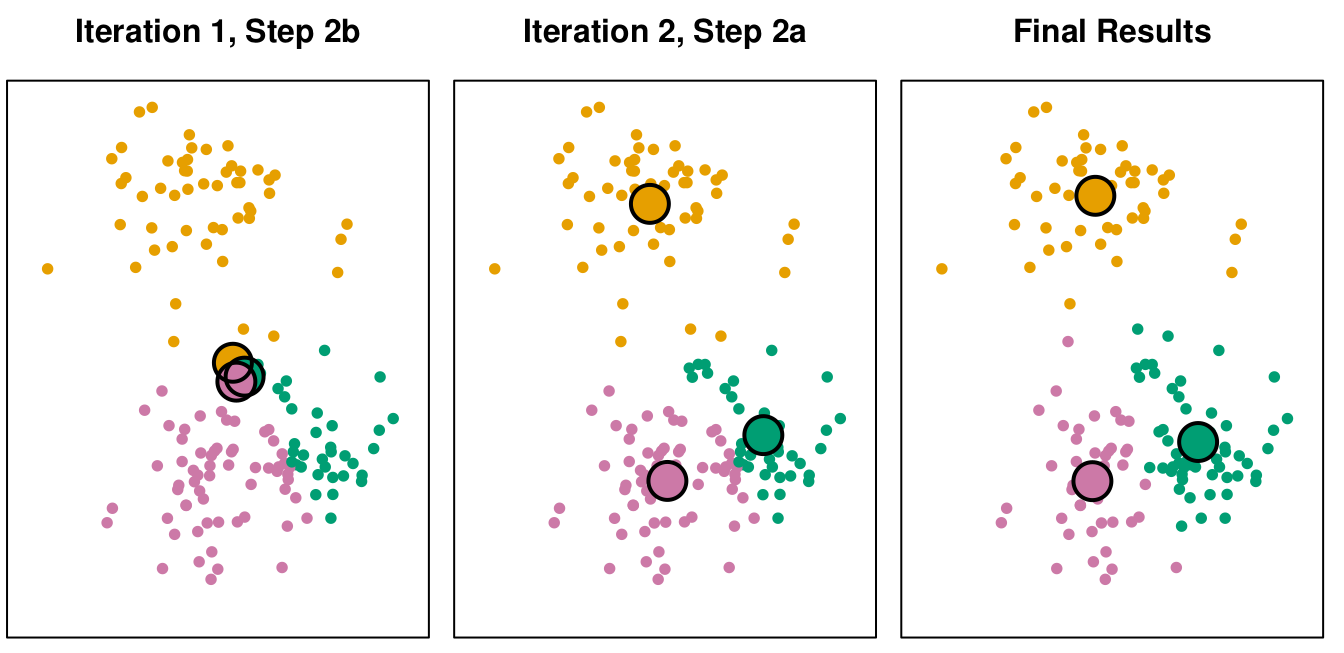
\includegraphics[align = c, width = .45\textwidth]{Fig12-8b}

% \InstructorNotes{Last step is after 10 iterations}


% \end{frame}
% %--- Next Frame ---%
% \begin{frame}[t]{Why does this work?}
% \centering

% 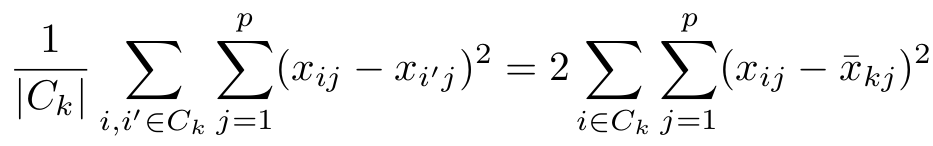
\includegraphics[align = c, width = .5\textwidth]{Eq12-18}
% where
% 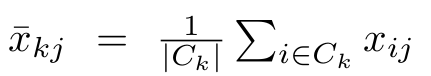
\includegraphics[align = c, width = .3\textwidth]{Eq12-18b}



% \begin{columns}
% \column{.45\textwidth}
% \centering
% \InstructorList{
%   \item Step 2a: cluster means are the constants that minimize the sum of squared deviations
% 	\item Step 2b: Reallocating observations can only decrease above equation value
% 	\item This means that algorithm will always find a local optimum
% }






% \column{.45\textwidth}
% \centering
% 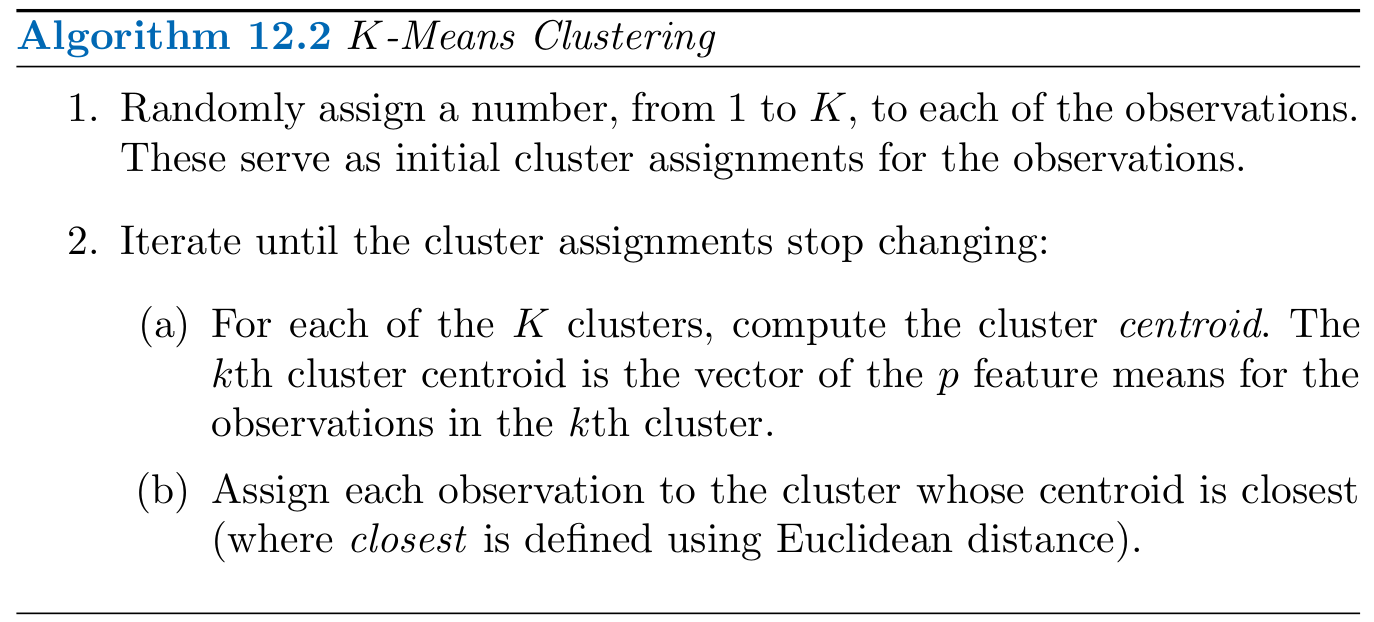
\includegraphics[align = c, width = \textwidth]{Alg12-2}



% \end{columns}

% \end{frame}
% %--- Next Frame ---%
% \begin{frame}[t]{Dependence on initial conditions}

% \begin{columns}
% \column{.45\textwidth}
% \centering
% 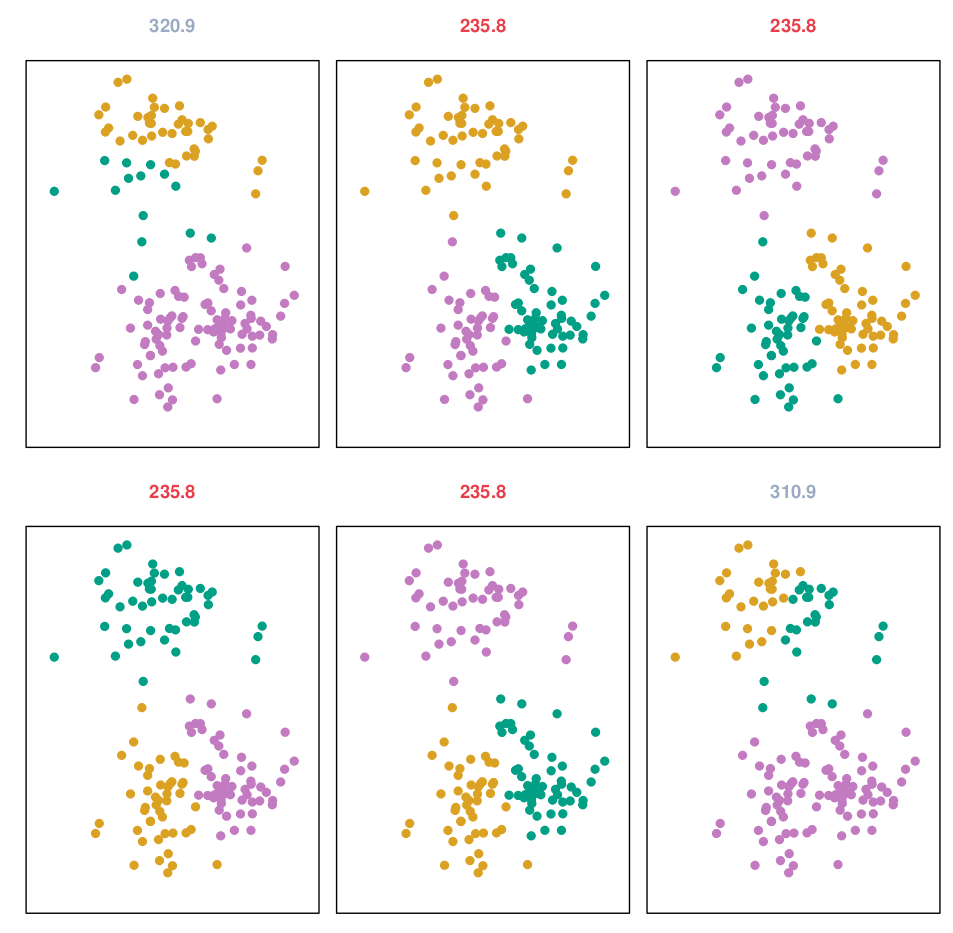
\includegraphics[align = c, width = \textwidth]{Fig12-9}



% \column{.45\textwidth}
% \centering
% \InstructorList{
%   \item Value is dependent on the randomly chosen starting point
% 	\item Figure has results from multiple runs
% 	\item Above each plot is the objective score
% 	\item Ones labeled in red all have the same best solution (even though diff colors)
% }



% \end{columns}

% \end{frame}
% %--- Next Frame ---%
% \begin{frame}[t]{Pros \& Cons of K-Means}

% \begin{columns}
% \column{.45\textwidth}
% \centering
% \textbf{Pros}
% \InstructorList{
%   \item Simple mathematical idea
% }



% \column{.45\textwidth}
% \centering
% \textbf{Cons}
% \InstructorList{
%   \item Need to choose $K$ in advance
% 	\item Doesn't always find the global minimum (can be mitigated by multiple runs)
% }




% \end{columns}

% \end{frame}
% %--- Next Frame ---%

%======================
%=================
\section{Hierarchical Clustering}
%=================




\begin{frame}[t]{Dendrogram}

\centering
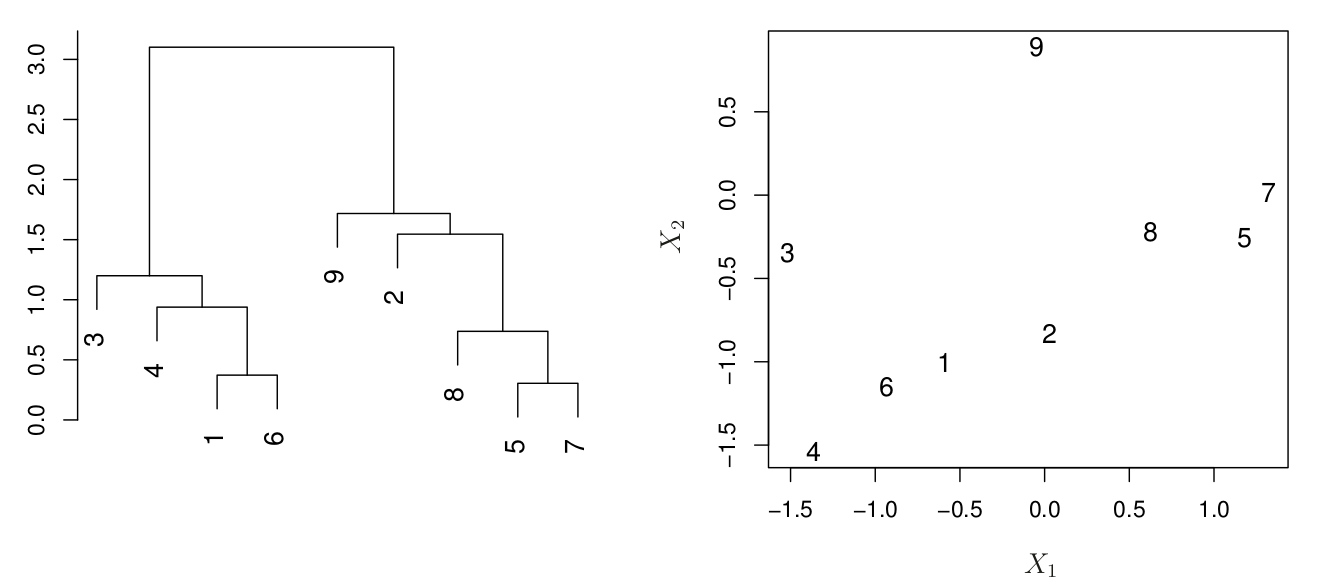
\includegraphics[align = c, width = .8\textwidth]{Fig12-12}

\InstructorList{
  \item Bottom-up agglomeration from each point
  \item Note the horizontal axis doesn't matter, could redraw
	\item R draws leaves with same length, not at zero (blech)
	\item WARNING: This is NOT single linkage
}


\end{frame}
%--- Next Frame ---%
\begin{frame}[t]{A bigger example }

\begin{columns}
\column{.45\textwidth}
\centering
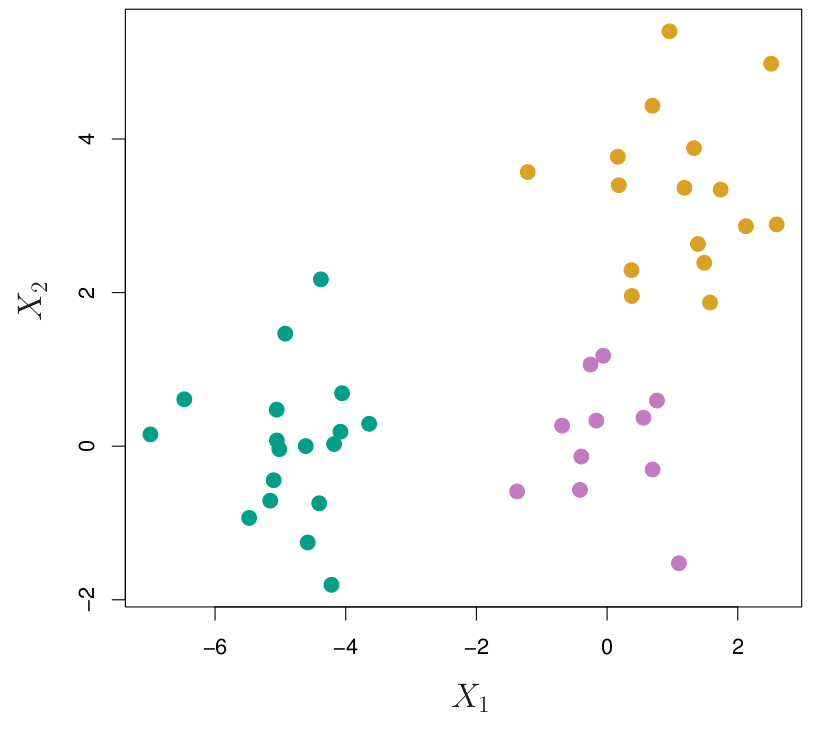
\includegraphics[align = c, width = \textwidth]{Fig12-10}

\InstructorList{
  \item Data generated with three labels
  \item Pretend you can't see the colors
}





\column{.28\textwidth}
\centering
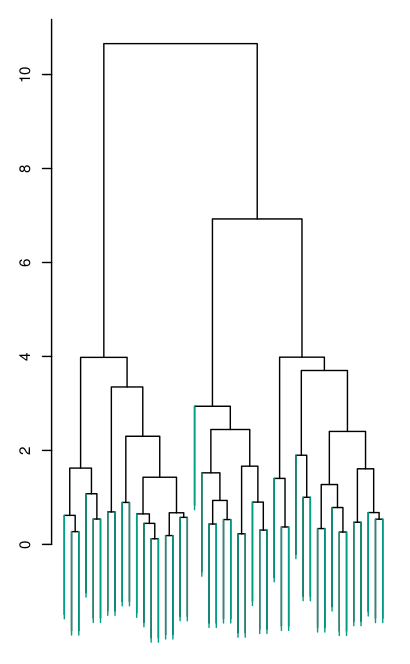
\includegraphics[align = c, width = \textwidth]{Fig12-11a}




\end{columns}

\end{frame}
%--- Next Frame ---%

\begin{frame}[t]{Single linkage}
\centering

Distance between cluster $A$ and cluster $B$:\\
Smallest distance between the points
\begin{equation*}
	L(A,B)= \min_{a \in A, b\in B}\|a-b\|
\end{equation*}


\begin{columns}
\column{.3\textwidth}

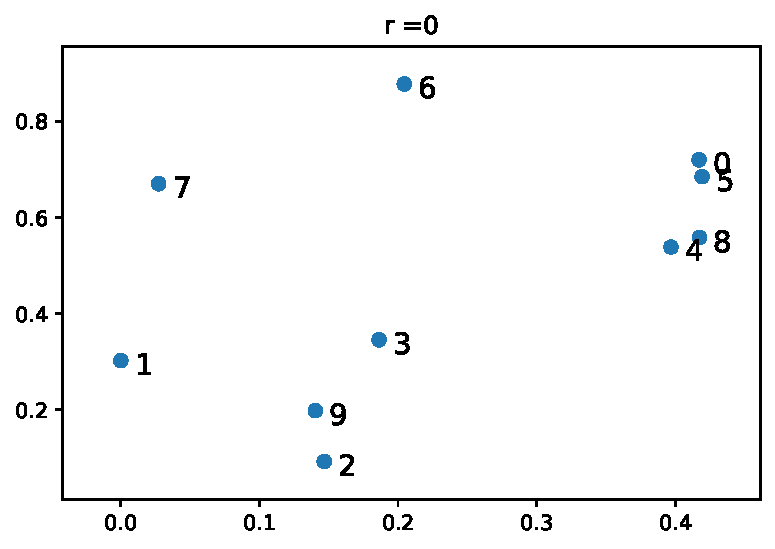
\includegraphics[align = c, width = \textwidth]{SingleLink-0p0.pdf}
\column{.3\textwidth}
\centering

\includegraphics[align = c, width = \textwidth]{SingleLink-Distance.pdf}

\end{columns}
\end{frame}
%--- Next Frame ---%

\begin{frame}[t]{Building the dendrogram}
\begin{columns}
\column{.3\textwidth}
\centering

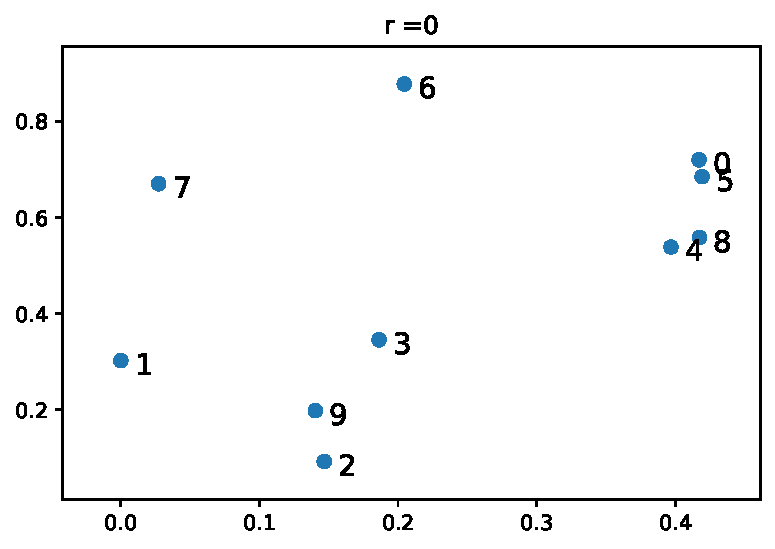
\includegraphics[align = c, width = \textwidth]{SingleLink-0p0.pdf}
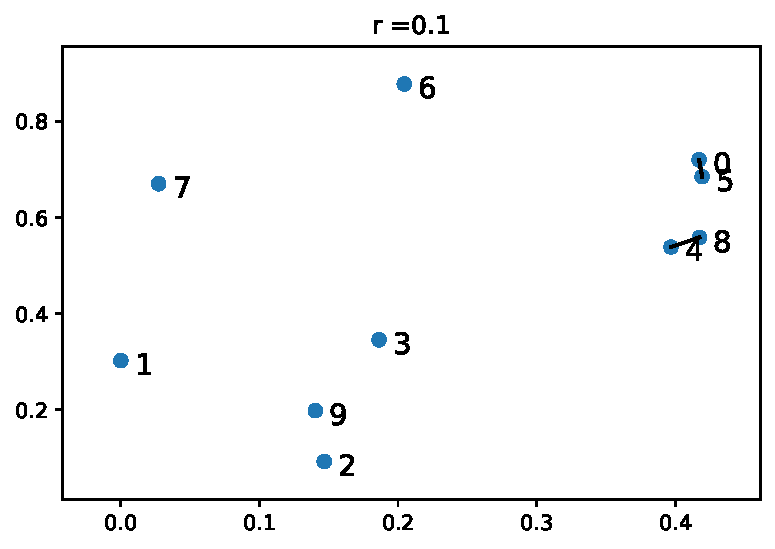
\includegraphics[align = c, width = \textwidth]{SingleLink-0p10.pdf}
\column{.3\textwidth}
\centering
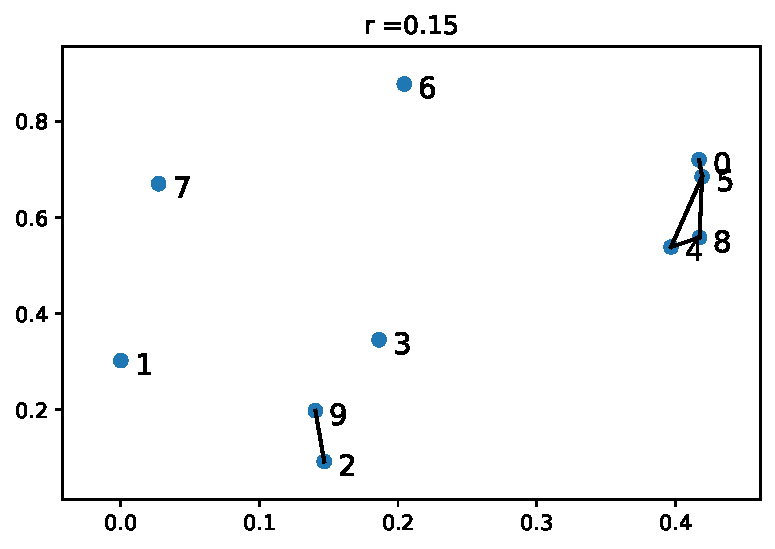
\includegraphics[align = c, width = \textwidth]{SingleLink-0p15.pdf}
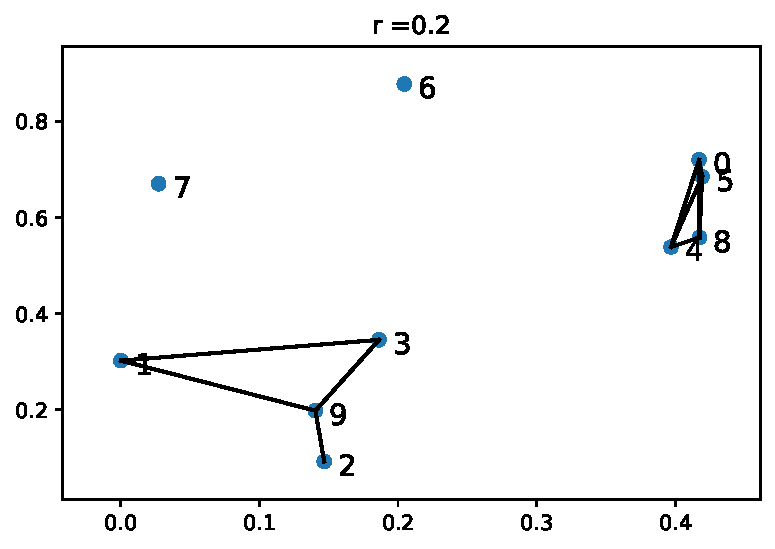
\includegraphics[align = c, width = \textwidth]{SingleLink-0p20.pdf}
\column{.3\textwidth}
\centering
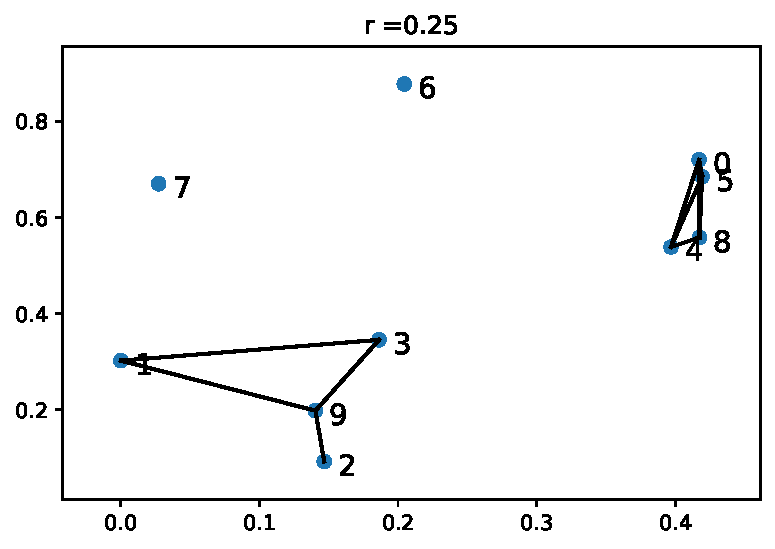
\includegraphics[align = c, width = \textwidth]{SingleLink-0p25.pdf}
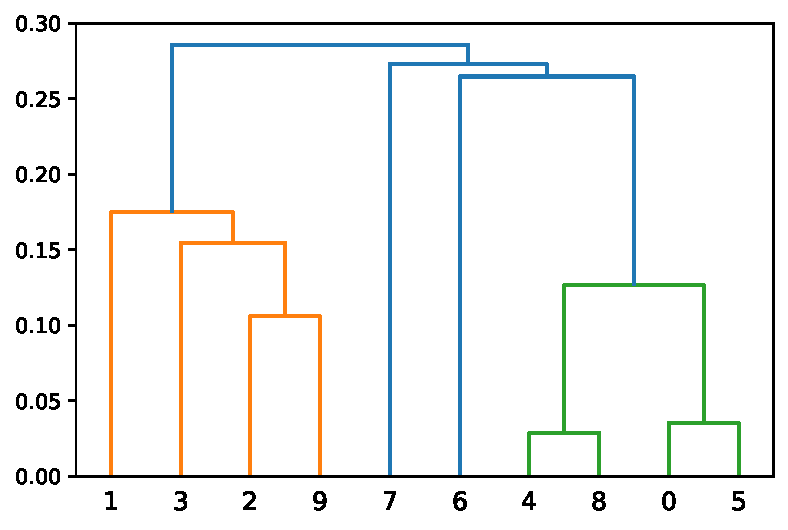
\includegraphics[align = c, width = \textwidth]{SingleLink-Dendrogram}

\end{columns}
\end{frame}
%--- Next Frame ---%




\begin{frame}[t]{How to get clusters}

\begin{columns}
\column{.45\textwidth}
\centering
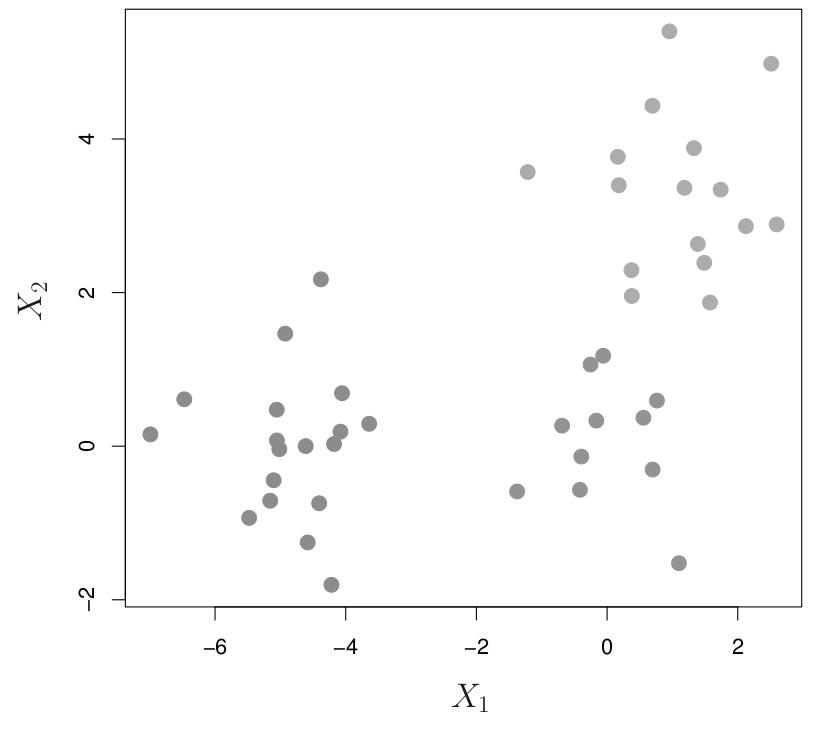
\includegraphics[align = c, width = \textwidth]{Fig12-10-BW}



\column{.28\textwidth}
\centering
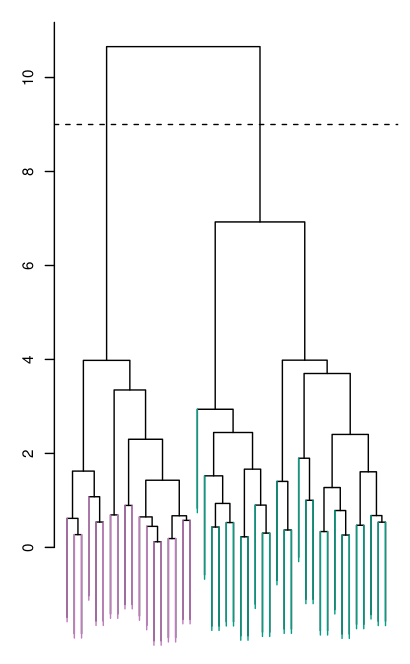
\includegraphics[align = c, width = \textwidth]{Fig12-11b}




\end{columns}

\end{frame}
%--- Next Frame ---%



\begin{frame}[t]{How to get different clusters}

\begin{columns}
\column{.45\textwidth}
\centering
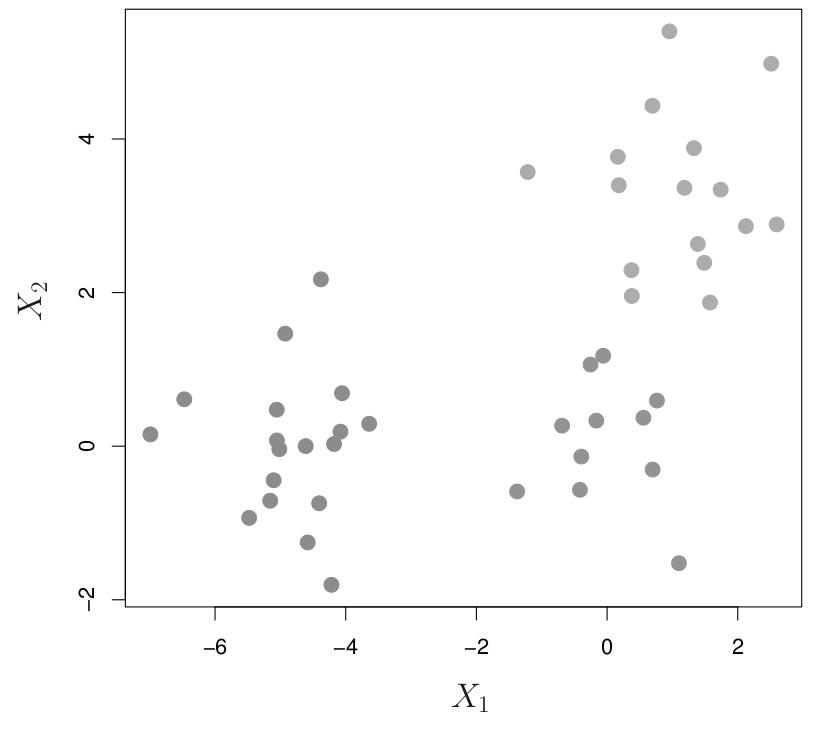
\includegraphics[align = c, width = \textwidth]{Fig12-10-BW}



\column{.28\textwidth}
\centering
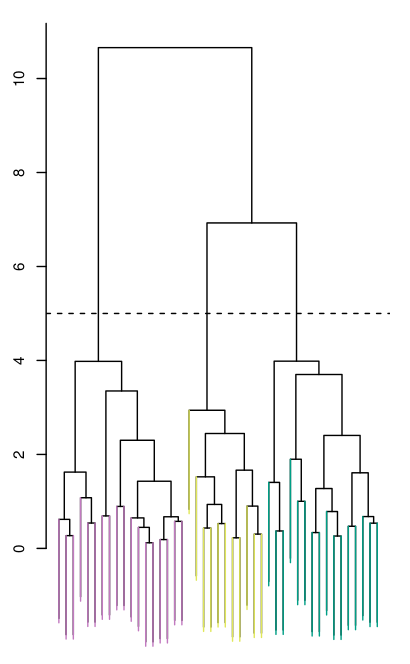
\includegraphics[align = c, width = \textwidth]{Fig12-11c}




\end{columns}

\end{frame}
%--- Next Frame ---%

\begin{frame}[t]{Can get any number of clusters}



\begin{columns}
\column{.45\textwidth}
\centering
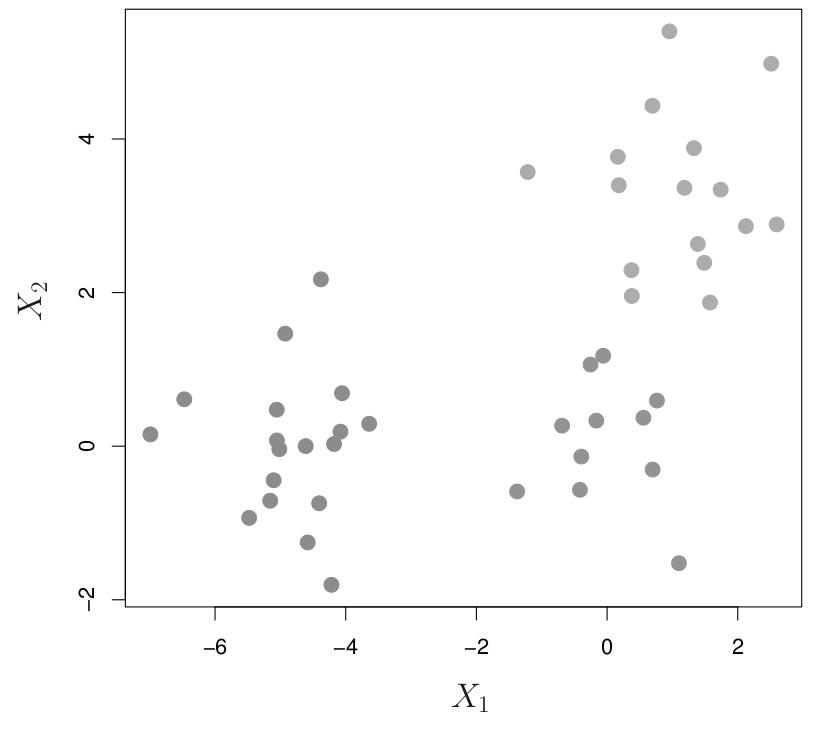
\includegraphics[align = c, width = \textwidth]{Fig12-10-BW}



\column{.28\textwidth}
\centering
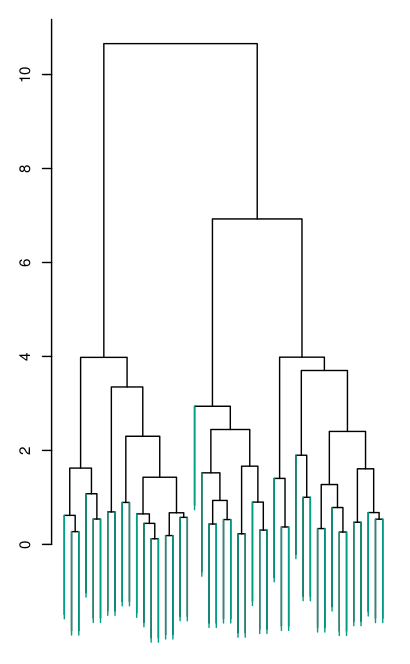
\includegraphics[align = c, width = \textwidth]{Fig12-11a}




\end{columns}

Test your understanding: \href{https://PollEv.com/clickable_images/mvuvAUIKxYGp5iSy22mY6/respond}{PollEv}


\end{frame}
%--- Next Frame ---%
% \begin{frame}[t]{Pros \& Cons of Hierarchical Clustering}
%
% \begin{columns}
% \column{.45\textwidth}
% \centering
% \textbf{Pros:}
% \InstructorList{
%   \item Can have any number of clusters
% 	\item Visualization by dendrogram
% }
%
%
% \column{.45\textwidth}
% \centering
% \textbf{Cons:}
% \InstructorList{
%   \item Cluster options must be nested
% 	\item Some things to pick.....
% }
%
%
% \end{columns}
%
% \end{frame}
%--- Next Frame ---%

\begin{frame}[t]{Linkage}

\begin{columns}
\column{.45\textwidth}
\centering
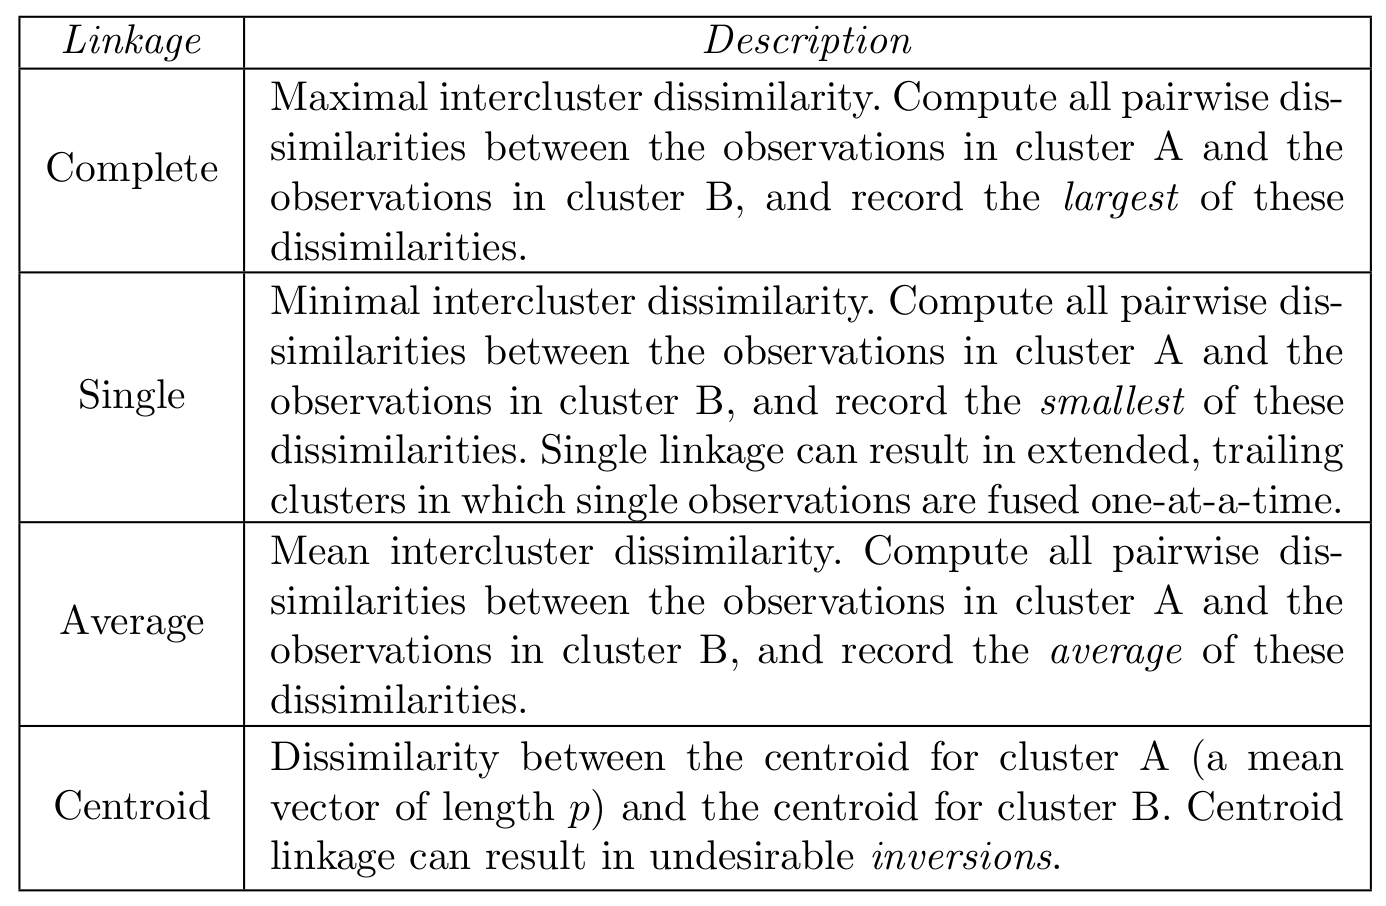
\includegraphics[align = c, width = \textwidth]{Table12-3}

\column{.45\textwidth}
\centering
\InstructorList{
  \item How do we talk about distance between clusters?
	\item Four most common ways to compare two clusters is at left
	\item Avg and complete linkage have more balanced dendrograms than single linkage
	\item Centroid shows up in genomics, but can create inversion, where two clusters fused at height below either of the individual clusters
}


\end{columns}

\end{frame}
%--- Next Frame ---%

\begin{frame}[t]{Example with complete linkage}

\begin{columns}
\column{.45\textwidth}
\centering
\includegraphics[align = c, width = .5\textwidth]{Fig12-12a}

Distance between cluster $A$ and cluster $B$:\\
\textbf{Largest} distance between the points
\begin{equation*}
	L(A,B)= \max_{a \in A, b\in B}\|a-b\|
\end{equation*}


\column{.45\textwidth}
\centering
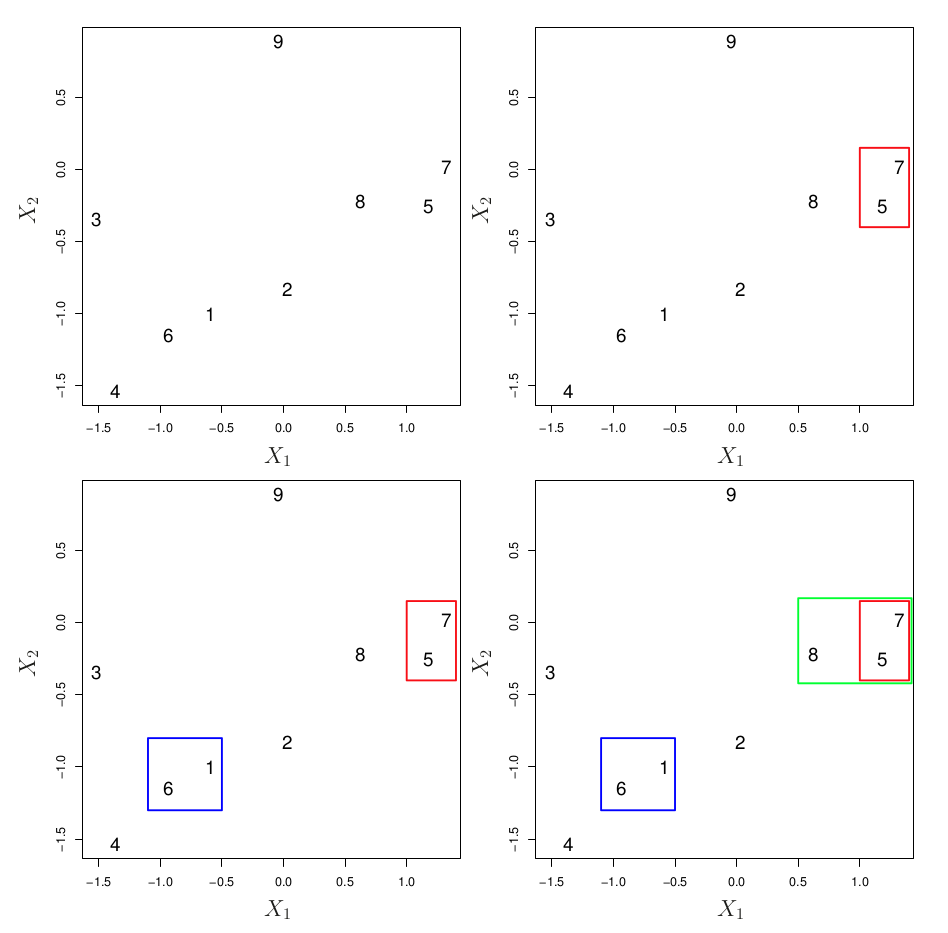
\includegraphics[align = c, width = \textwidth]{Fig12-13}

\end{columns}

\end{frame}
%--- Next Frame ---%
\begin{frame}[t]{Examples of different linkage }

\centering
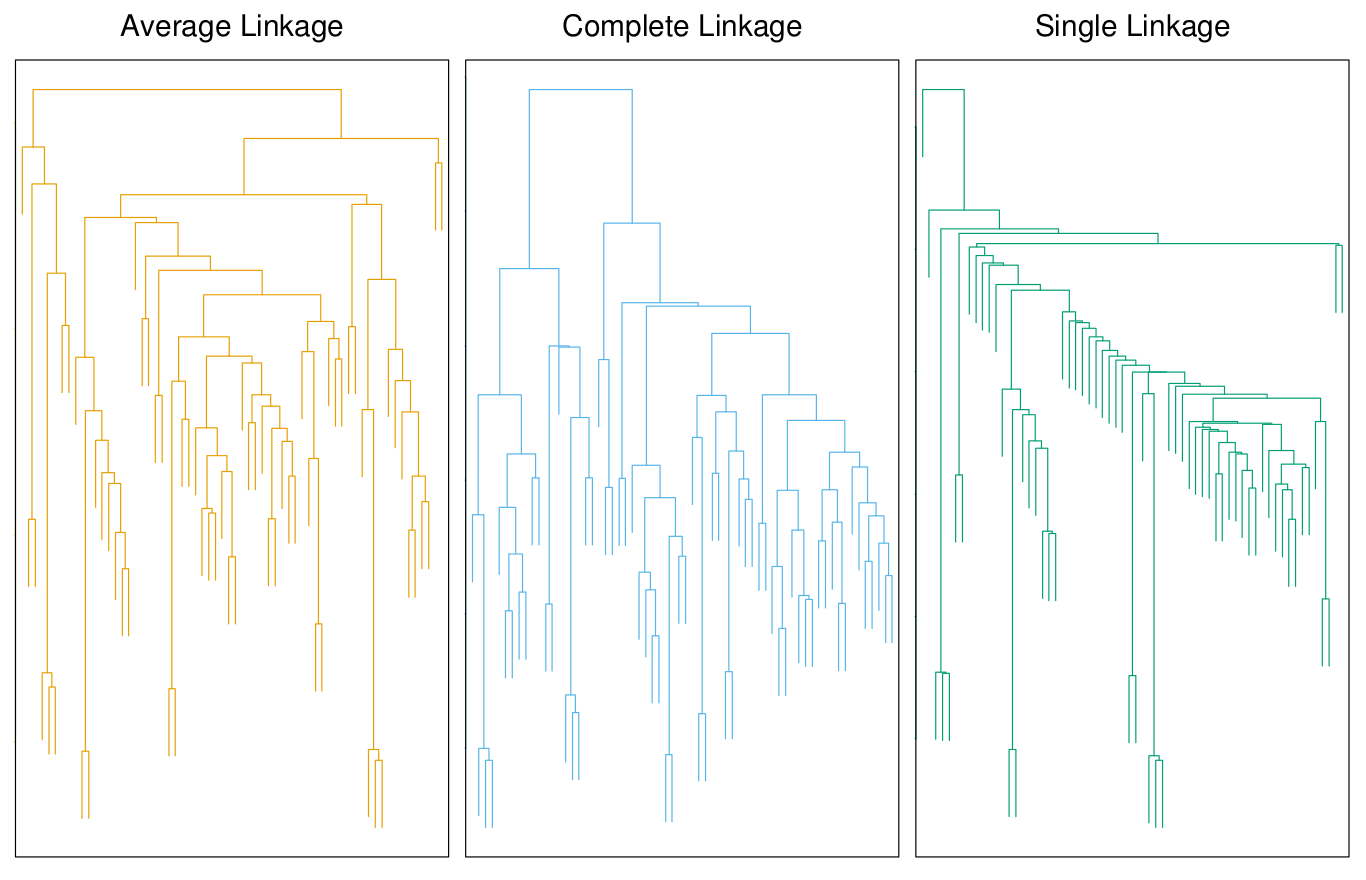
\includegraphics[align = c, width = .7\textwidth]{Fig12-14}



\end{frame}
%--- Next Frame ---%
\begin{frame}[t]{Dependence on dissimilarity measure}
\begin{columns}
\column{.45\textwidth}
\centering

\InstructorList{
  \item Choice of comparison is context dependent
	\item Result of clustering depends on the distance you choose
	\item these ``distance'' carries assumptions about the shape of the underlying space. (pieces cutout or distortef)
}


\column{.45\textwidth}
\centering

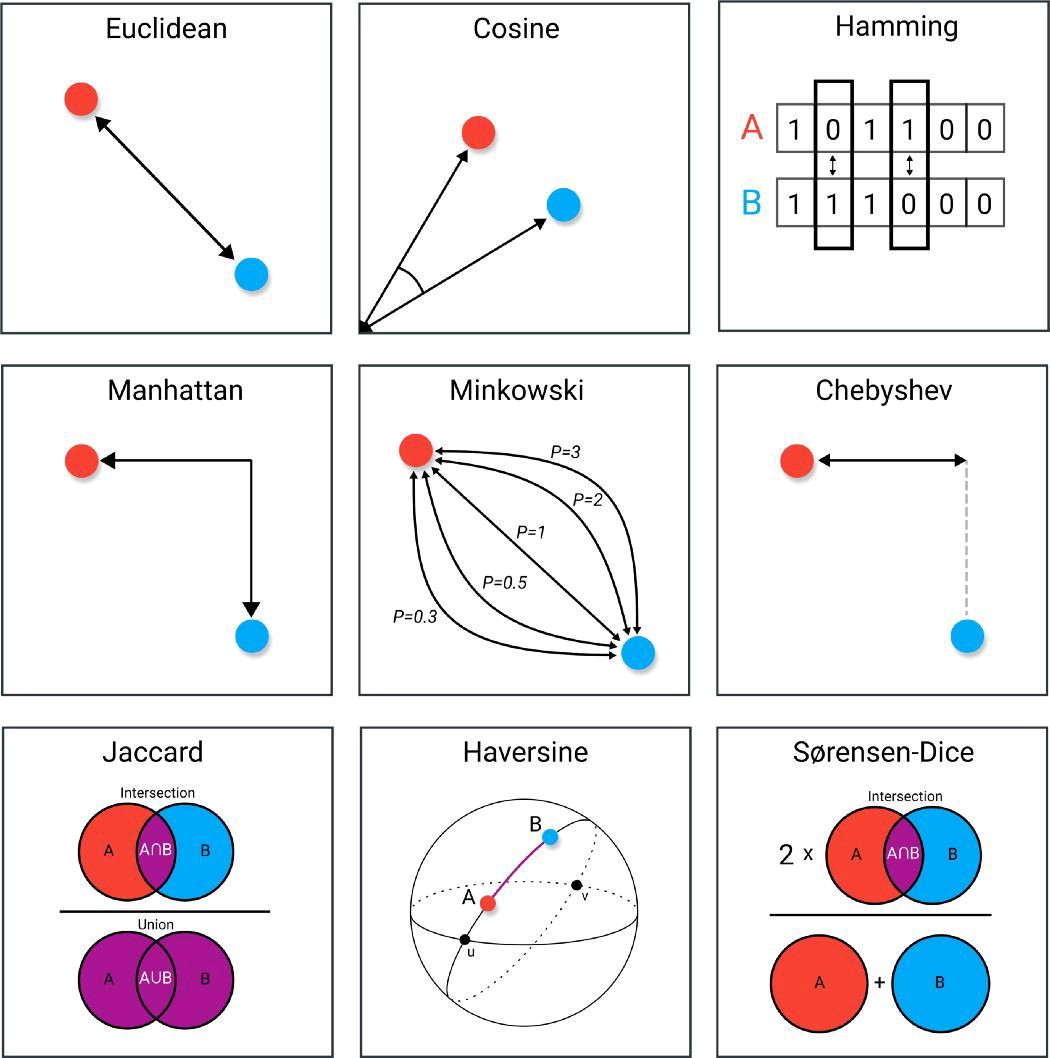
\includegraphics[align=c, width = \textwidth]{Clustering-DistanceTweet-JustFig.jpeg}
\href{https://twitter.com/UsmanKayaniPhD/status/1518243229832994818}{Photo Credit Link}
\end{columns}

\end{frame}
%--- Next Frame ---%
{
\setbeamercolor{background canvas}{bg=Apricot!25}
\begin{frame}[t]{Coding}
\begin{columns}
\column{.45\textwidth}
\centering
\column{.45\textwidth}
\centering
\end{columns}
\end{frame}
}
%--- Next Frame ---%
% \begin{frame}[t]{Example with shopping}
%
% \begin{columns}
% \column{.45\textwidth}
% \centering
% \InstructorList{
%   \item Goal is to find similar shoppers
% 	\item Pretend this is \# purchases of particular item
% 	\item Using euclidean distance, 2 and 3 are very similar, and 1 is very different
% 	\item If using correlation-based distance, they're all similar
% }
%
%
% \column{.45\textwidth}
% \centering
% 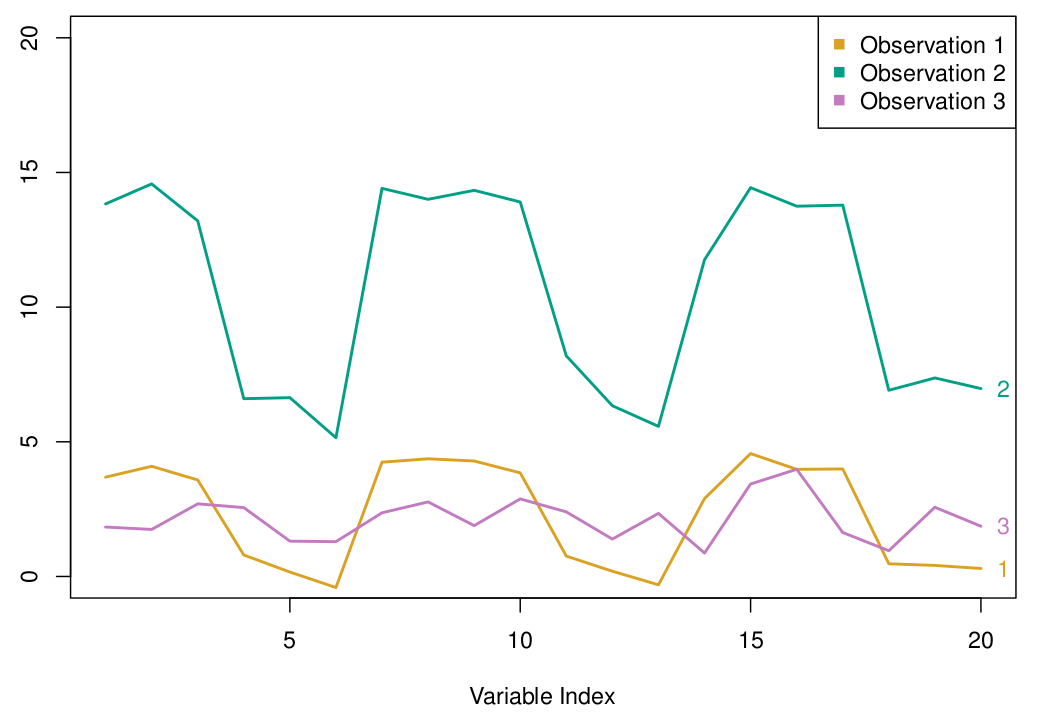
\includegraphics[align = c, width = \textwidth]{Fig12-15}
%
% \end{columns}
%
% \end{frame}
% %--- Next Frame ---%
% \begin{frame}[t]{Whether or not to scale}
%
% \begin{columns}
% \column{.45\textwidth}
% \centering
% \InstructorList{
%   \item Scaling variables could help (or not)
% 	\item Example is shopping where one big purchase (computer) might outweight smaller, for better or worse
% 	\item Each shopper shown in diff color
% 	\item Left raw. Middle scale variables by std dev. Right scale dollars spent.
% }
%
%
% \column{.45\textwidth}
% \centering
% 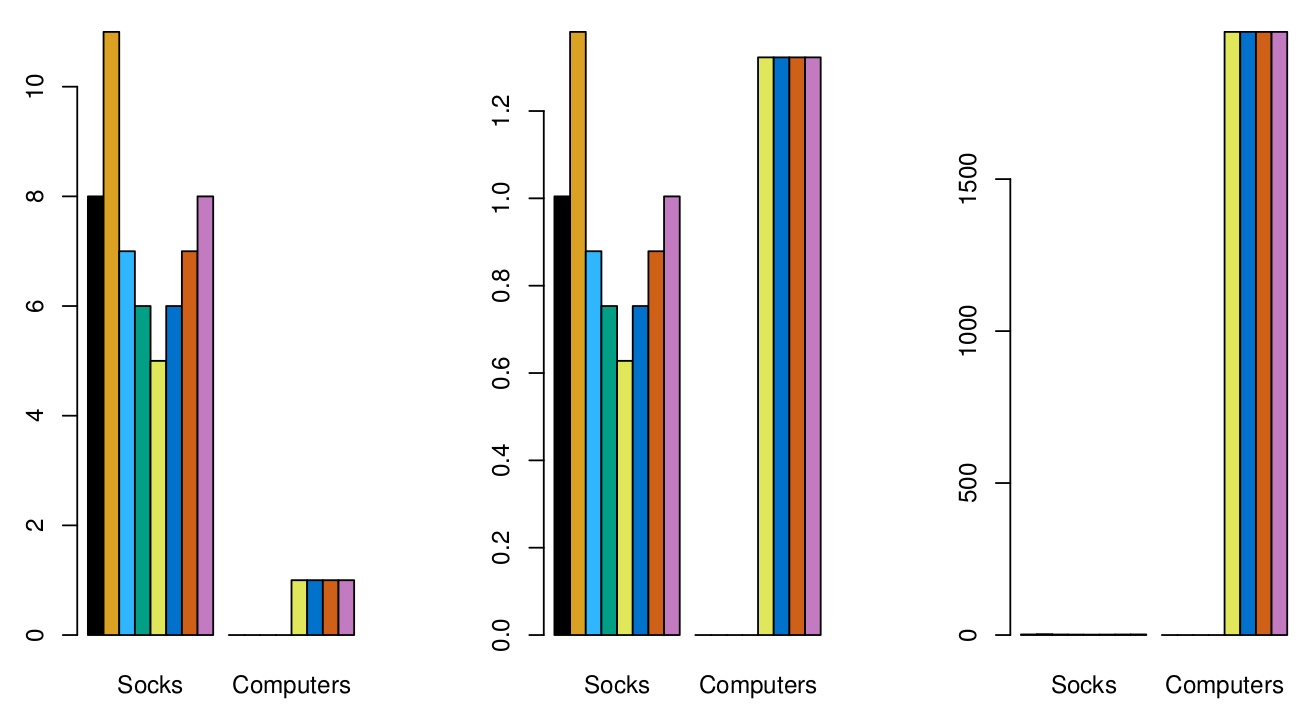
\includegraphics[align = c, width = \textwidth]{Fig12-16}
%
% \end{columns}
%
% \end{frame}
% %--- Next Frame ---%

%======================

%--- Next Frame ---%

\begin{frame}[t]{Next time}


	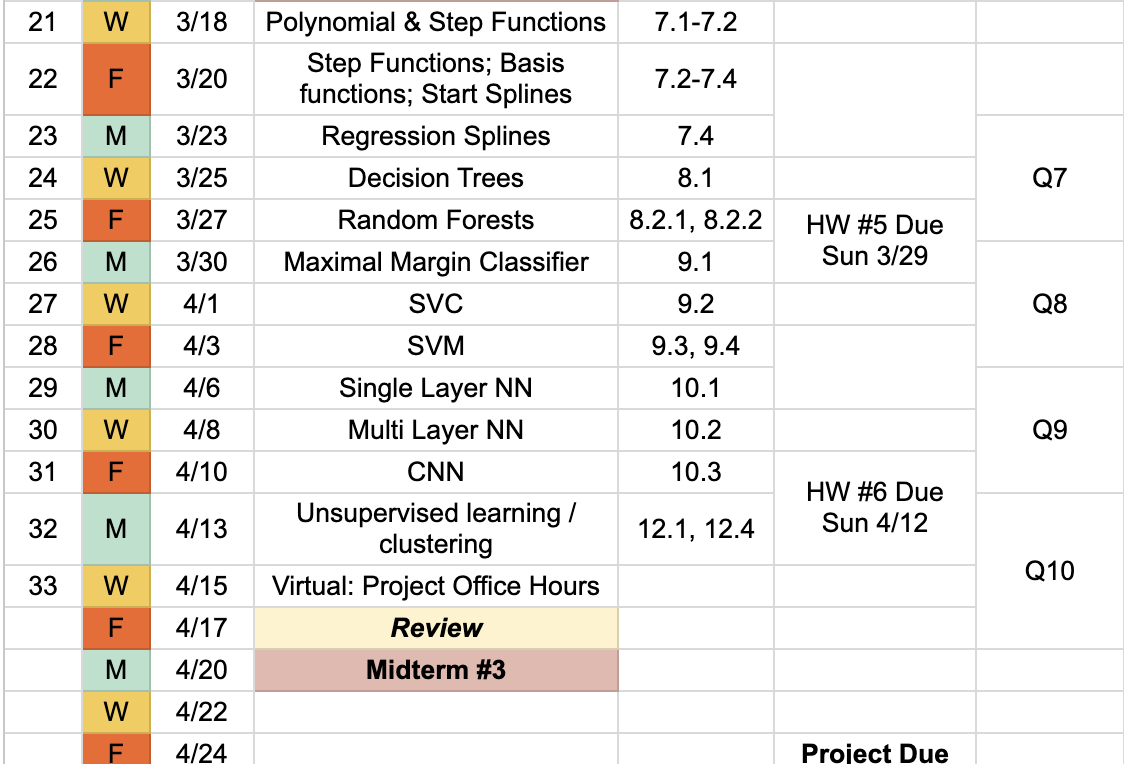
\includegraphics[align = c, width = .45\textwidth]{Schedule-S26-3.png}
	
% Q of the Day: What is the difference between single and complete linkage? 

\end{frame}

\end{document}
